\let\negmedspace\undefined
\let\negthickspace\undefined
\documentclass[journal]{IEEEtran}
\usepackage[a5paper, margin=10mm, onecolumn]{geometry}
\usepackage{lmodern} 
\usepackage{tfrupee} 
\setlength{\headheight}{1cm}
\setlength{\headsep}{0mm}   

\usepackage{gvv-book}
\usepackage{gvv}
\usepackage{cite}
\usepackage{amsmath,amssymb,amsfonts,amsthm}
\usepackage{algorithmic}
\usepackage{graphicx}
\usepackage{textcomp}
\usepackage{xcolor}
\usepackage{txfonts}
\usepackage{listings}
\usepackage{enumitem}
\usepackage{mathtools}
\usepackage{gensymb}
\usepackage{comment}
\usepackage[breaklinks=true]{hyperref}
\usepackage{tkz-euclide} 
\usepackage{listings}                             
\def\inputGnumericTable{}                                 
\usepackage[latin1]{inputenc}                                
\usepackage{color}                                            
\usepackage{array}                                            
\usepackage{longtable}                                       
\usepackage{calc}                                             
\usepackage{multirow}                                         
\usepackage{hhline}                                           
\usepackage{ifthen}                                           
\usepackage{lscape}
\usepackage{xparse}

\bibliographystyle{IEEEtran}

\title{3.2.3}
\author{EE25BTECH11062 - Vivek K Kumar}

\begin{document}
\maketitle

\renewcommand{\thefigure}{\theenumi}
\renewcommand{\thetable}{\theenumi}

\numberwithin{equation}{enumi}
\numberwithin{figure}{enumi} 

\textbf{Question}:\\
Draw a parallelogram ABCD in which $BC = 5cm, AB = 3cm$ and $\angle ABC = 60\degree$, divide it into triangles ACB and ABD by the diagonal BD

\textbf{Solution: }

Let $\vec{A}$, $\vec{B}$, $\vec{C}$ and $\vec{D}$ represent position vectors of the vertices of parallelogram.

Given information, 
\begin{align}
\norm{\vec{A-B}} &= 3 \\
\norm{\vec{C-B}} &= 5 \\
\angle B &= \frac{\pi}{3}
\end{align}

The coordinates of $\vec{A}, \vec{B}, \vec{C}$ can be expressed as
\begin{align}
\vec{B} &= \myvec{0\\0} \\
\vec{C} &= \norm{\vec{C-B}}\myvec{1\\0} \\
\vec{A} &= \norm{\vec{A-B}}\myvec{cosB\\sinB} 
\end{align}

Since $\vec{A}, \vec{B}, \vec{C}, \vec{D}$ form vertices of a parallelogram,
\begin{align}
\frac{\vec{A}+\vec{C}}{2} &= \frac{\vec{B}+\vec{D}}{2} \\
\vec{D} &= \vec{A+C-B}\\
\vec{D} = \norm{\vec{A}-\vec{B}}\myvec{cosB\\sinB} &+  \norm{\vec{C}-\vec{B}}\myvec{1\\0} - \myvec{0\\0}
\end{align}
\\
Substituting values, 
\begin{align}
    \vec{A} &= \myvec{3/2 \\ 3\sqrt{3}/{2}} \\
    \vec{B} &= \myvec{0 \\ 0} \\
    \vec{C} &= \myvec{5 \\ 0} \\
    \vec{D} &= \myvec{13/2 \\ 3\sqrt{3}/2}
\end{align}
\begin{table}[H]    
  \centering
  \begin{tabular}{|c|c|}
\hline
\textbf{Name} & \textbf{Value} \\ \hline
$\vec{A}$ & $\myvec{2 & 1 \\0 & 3}$ \\ \hline
\end{tabular}

  \caption{Coordinates of the vertices of parallelogram}
  \label{tab:3.2.3}
\end{table}




\begin{figure}[H]
   \centering
  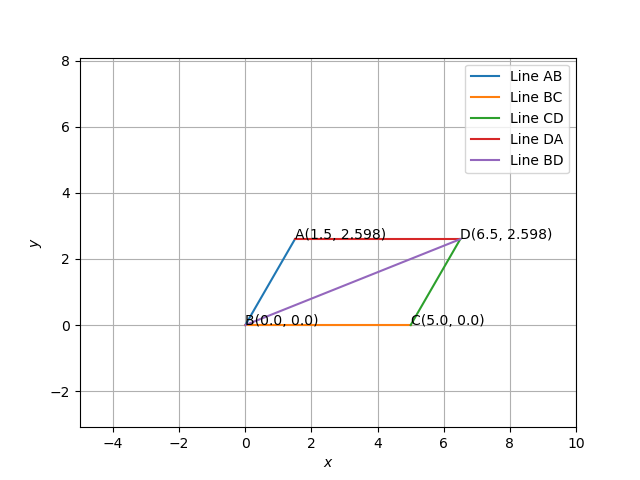
\includegraphics[width=0.64\columnwidth]{figs/fig.png}
   \caption{Given parallelogram split across BD}
   \label{stemplot}
\end{figure}
\end{document}  


